\chapter{Environment Influence } 
Not just the sample rate and error is determining factors when designing a \ab{NILM} application. The environment which the application is deployed and trained in is critical for the performance of the system. 

The environment is the parameters describing the static conditions of the household which the algorithms is deployed in. An example of an environment parameter can be number of known devices, number of unknown devices, number of simultaneously active devices or number of training days. In order to investigate some of the environment parameters effect the SmartHG dataset is used. 

\section{Challenges In The SmartHG Dataset} 
The \ab{ECO} dataset, consists of 6 households and the data is sampled at a rate of 1 Hz over a period of 8 months. The SmartHG dataset is different in many aspects. The data is sampled at a slower rate of $\frac{1}{30}$ Hz, but on 25 households over a period of 6 month. Each house have only a small number of sub-meters. The sub-meters is mainly placed on little consumers such as televisions and stereos, which presents an interesting challenge for load disaggregation. The SmartHG dataset contains both the aggregated data, and the instantaneous power usages of the different households.

\begin{figure}[H]
\centering
\includegraphics[width=1\textwidth]{billeder/TotalPie.png}
\caption{Frequency comparison of the reconstruction methods}
\label{fig:SLC}
\end{figure}

In figure \ref{fig:SLC} is the power distribution of three households shown. This illustrates how much energy each appliance uses, in relation to the households total energy consumption. The Other category shows the energy consumption not accounted for by the sub-meters.  

Household 3,10 and 18 is some of the houses that have the smallest "other" category. They are therefore selected for further study, since they provide the most information about the house. 

\section{Appliance Noise Influence On Detection }
\label{sec:AppNoise}
The households in the SmartHG dataset have a relative big consumption created by other appliances than the ones with a sub-meter. The consumption can be thought of as "appliance noise", since it is a signal that is not included in the disaggregation model. 

\subsection{Detection In A Noisy Environment }
\label{sec:NOISE}
To investigate the influence appliance noise have on a \ab{NILM} application, disaggregation of the known appliances of house 3, 10 and 18 is done using the Parson and \ab{FHMM} algorithm. 

\begin{table}[H]                             
\centering                                   
\begin{tabular}{cc|c|c|c|c|}
\cline{3-6}
\multicolumn{1}{l}{}                            &        & \multicolumn{2}{c|}{FHMM} & \multicolumn{2}{c|}{Parson} \\ \cline{3-6} 
\multicolumn{1}{l}{}                            &        & F1        & Accuracy      & F1         & Accuracy       \\ \hline
\multicolumn{1}{|c|}{\multirow{3}{*}{House 3}}  & TV 1   & 0.19      & 0.74          & 0.10       & 0.40           \\ \cline{2-6} 
\multicolumn{1}{|c|}{}                          & PC     & 0.19      & 0.84          & 0.13       & 0.45           \\ \cline{2-6} 
\multicolumn{1}{|c|}{}                          & TV 2   & 0.03      & 0.84          & 0.20       & 0.11           \\ \hline
\multicolumn{1}{|c|}{\multirow{4}{*}{House 10}} & TV 1   & 0.60      & 0.76          & 0.40       & 0.25           \\ \cline{2-6} 
\multicolumn{1}{|c|}{}                          & Stereo & -         & 1.00          & -          & 1.00           \\ \cline{2-6} 
\multicolumn{1}{|c|}{}                          & PC     & -         & 0.99          & -          & 0.99           \\ \cline{2-6} 
\multicolumn{1}{|c|}{}                          & TV 2   & -         & 0.99          & -          & 0.99           \\ \hline
\multicolumn{1}{|c|}{\multirow{3}{*}{House 18}} & TV 1   & 0.36      & 0.65          & 0.24       & 0.14           \\ \cline{2-6} 
\multicolumn{1}{|c|}{}                          & Lamp   & -         & 0.99          & -          & -              \\ \cline{2-6} 
\multicolumn{1}{|c|}{}                          & TV 2   & 0.73      & 0.58          & -          & 0.00           \\ \hline
\end{tabular}                               
\caption{Appliance disaggregation results of house 3,10 and 18 for the SmartHG dataset.}                     
\label{table:Tab:SHGREAL}                    
\end{table}                   

On table \ref{table:Tab:SHGREAL} is the results from the disaggregation shown. The low F1 scores indicates that it is hard for the algorithms to correctly disaggregate the meters. This is due to the many spikes there are in the data that can indicate a change in appliance usage. On figure \ref{fig:RMD} is a sample from the validation period shown. The blue line shows the data from the main meter. The other lines indicates the appliances. On the left side of the figure is the true consumption shown for all the meters. This consumption is known from the sub-meters on the appliances. On the right side is the true main meter signal shown, and the inferred usages of the different appliances created by the \ab{FHMM} algorithm. 

\begin{figure}[H]
\begin{picture}(0,150)
\put(0,10){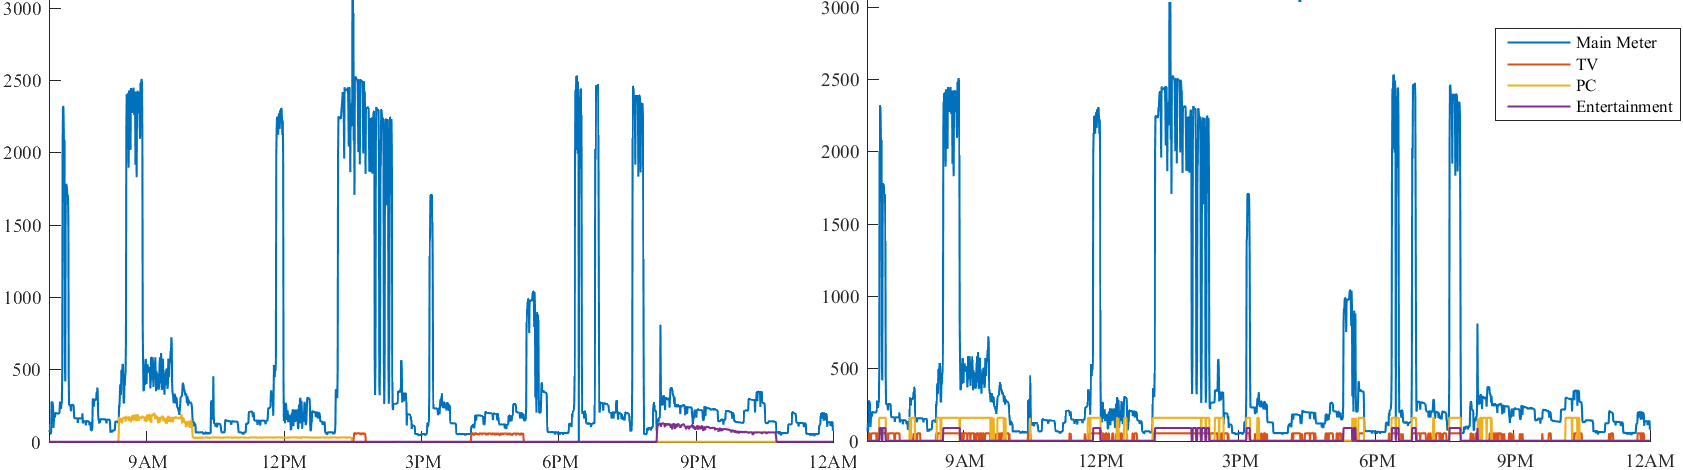
\includegraphics[width=1\textwidth]{billeder/RecognitionEx1.png}}

\put(90,140){True Signals}
\put(300,140){Inferred Signal}

\put(-10,65){\rotatebox{90}{Watt}}
\put(215,0){Time}

\end{picture}
\caption{FHMM disaggregation snippet}
\label{fig:RMD}
\end{figure}

On the figure it is shown how the main meter have many fluctuations. The algorithm tries to map each fluctuation to a change in a appliance, or noise. There are many of the noise fluctuations that are similar to the appliance changes, and this creates errors in the disaggregation. 

\subsection{Detection In Noise Free Environment }
\label{sec:NOISEFREE}
The assumption that the noise is what troubles the disaggregation, dictates that for a house where all appliances are known, and therefore there are no noise, will preform better. 

\begin{figure}[H]
\centering
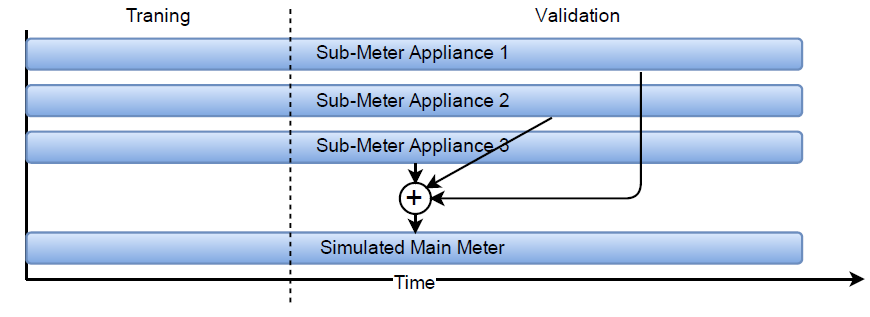
\includegraphics[width=1\textwidth]{billeder/SimIllu.png}
\caption{Artificially constructed main meter}
\label{fig:SIL}
\end{figure}

In order to test this hypothesis was an main meter signal artificially constructed by summing the values of all the sub-meters in a house as illustrated on figure \ref{fig:SIL}. In this manner was a new set of artificial houses created where there where no appliance noise. By applying the same disaggregation algorithms as for the noisy environment on the noise free environment it is seen that the disaggregation is much higher as shown in table \ref{table:Tab:SHGSIM}.

\begin{table}[H]                             
\centering                                   
\begin{tabular}{cc|c|c|c|c|}
\cline{3-6}
                                                &        & \multicolumn{2}{c|}{FHMM} & \multicolumn{2}{c|}{Parson} \\ \cline{3-6} 
                                                &        & F1        & Accuracy      & F1         & Accuracy       \\ \hline
\multicolumn{1}{|c|}{\multirow{3}{*}{House 3}}  & TV 1   & 0.73      & 0.96          & 0.26       & 0.86           \\ \cline{2-6} 
\multicolumn{1}{|c|}{}                          & PC     & 0.74      & 0.96          & 0.30       & 0.91           \\ \cline{2-6} 
\multicolumn{1}{|c|}{}                          & TV 2   & 0.83      & 0.96          & 0.20       & 0.11           \\ \hline
\multicolumn{1}{|c|}{\multirow{4}{*}{House 10}} & TV 1   & 0.97      & 0.98          & 0.40       & 0.25           \\ \cline{2-6} 
\multicolumn{1}{|c|}{}                          & Stereo & -         & 1.00          & -          & 1.00           \\ \cline{2-6} 
\multicolumn{1}{|c|}{}                          & PC     & -         & 0.99          & -          & 0.99           \\ \cline{2-6} 
\multicolumn{1}{|c|}{}                          & TV 2   & -         & 0.99          & -          & 0.99           \\ \hline
\multicolumn{1}{|c|}{\multirow{3}{*}{House 18}} & TV 1   & 0.95      & 0.98          & 0.24       & 0.14           \\ \cline{2-6} 
\multicolumn{1}{|c|}{}                          & Lamp   & -         & 0.99          & -          & -              \\ \cline{2-6} 
\multicolumn{1}{|c|}{}                          & TV 2   & 0.73      & 0.58          & 0.73       & 0.58           \\ \hline
\end{tabular}                              
\caption{Disaggregation of appliances on artificially constructed main meters }                     
\label{table:Tab:SHGSIM}                     
\end{table}   

As shown on table \ref{table:Tab:SHGSIM} the F1 and accuracy score have both improved. Even though the artificial house only contains three or four appliances, and they are all accounted for by the model, there are still some of the appliances that are hard to find. This is due to the appliances power usage pattern in off/standby mode combine with the rare usage of the devices. When the standby pattern of a device is complex and the appliance is only rarely used the model will try to fit to the standby pattern and not the usage pattern, to get the most accurate consumption disaggregation. This can make the model incapable of detecting change between the on/off states.

One other aspect to note is that even though the F1 scores is higher, only a few is higher than 0.9. This is due to the similarity effect. When a house contains two or more appliances that are similar it gets harder for the algorithm to tell if it is the one or the other. This is what happens for TV 1 and TV 2 in house 3. The algorithms will wrongfully assign some of the events belonging to TV 1, to TV 2 and vice versa. This can be a problem if the goal is to determine exactly witch appliance there is responsible for the power consumption. This is one of the key aspects of the little consumers problem, discussed in chapter \ref{sec:AppRec}.

This has a profound effect on the parson algorithm that are designed to spilt up appliances based on appliance category's, by utilizing a set of general models. Since a lot of the appliances are similar in their consumption changes from state to state the parson models are almost identical which lead to the events being wrongly categorised. 

\newpage

\subsection{Noise Effect On Training And Validation }
The experiments the two previous sections \ref{sec:NOISE} and \ref{sec:NOISEFREE} suggest that appliance noise have an impact on the performance of the system. But for a system based on machine learning techniques like the \ab{FHMM} and the Parson algorithms it raises the questions is it to hard for the system to find the correct models in the noise, or are the noise just interfering with the correct models? 

\begin{figure}[H]
\centering
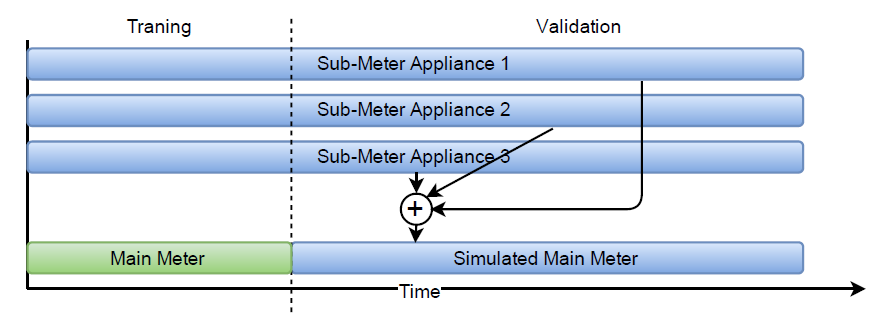
\includegraphics[width=1\textwidth]{billeder/REALSIM.png}
\caption{Illustration of dataset creation by combining real and constructed data}
\label{fig:REALSIMILU}
\end{figure}

In order to investigate these questions was a new dataset created that combined real data, collected from the house main meter, and an artificially constructed main meter. The new dataset was created by using the real data in the training period of the house, and using the constructed main meter in the validation, as illustrated on figure \ref{fig:REALSIMILU}.

This creates a very noisy environment in the training phase and a noise free environment in the validation phase. If the noise did not influence the creation of the statistical models that represent each appliance, then the results was expected to be just as good as for the noise free experiments conducted in section \ref{sec:NOISEFREE}.


\begin{table}[H]                             
\centering                                   
\begin{tabular}{cc|c|c|c|c|}
\cline{3-6}
\multicolumn{1}{l}{}                            &        & \multicolumn{2}{c|}{FHMM} & \multicolumn{2}{c|}{Parson} \\ \cline{3-6} 
\multicolumn{1}{l}{}                            &        & F1        & Accuracy      & F1         & Accuracy       \\ \hline
\multicolumn{1}{|c|}{\multirow{3}{*}{House 3}}  & TV 1   & 0.20      & 0.94          & 0.23       & 0.86           \\ \cline{2-6} 
\multicolumn{1}{|c|}{}                          & PC     & 0.29      & 0.94          & 0.32       & 0.92           \\ \cline{2-6} 
\multicolumn{1}{|c|}{}                          & TV 2   & 0.00      & 0.88          & 0.20       & 0.11           \\ \hline
\multicolumn{1}{|c|}{\multirow{4}{*}{House 10}} & TV 1   & 0.10      & 0.74          & 0.40       & 0.25           \\ \cline{2-6} 
\multicolumn{1}{|c|}{}                          & Stereo & -         & 1.00          & -          & 1.00           \\ \cline{2-6} 
\multicolumn{1}{|c|}{}                          & PC     & -         & 0.99          & -          & 0.99           \\ \cline{2-6} 
\multicolumn{1}{|c|}{}                          & TV 2   & -         & 0.99          & -          & 0.99           \\ \hline
\multicolumn{1}{|c|}{\multirow{3}{*}{House 18}} & TV 1   & 0.00      & 0.86          & 0.24       & 0.14           \\ \cline{2-6} 
\multicolumn{1}{|c|}{}                          & Lamp   & -         & 0.99          & -          & -              \\ \cline{2-6} 
\multicolumn{1}{|c|}{}                          & TV 2   & 0.73      & 0.58          & 0.73       & 0.58           \\ \hline
\end{tabular}                                
\caption{Disaggregation in real and constructed main meters combined.}                     
\label{table:Tab:SHGREALSIM}                 
\end{table}    

If the results from the experiment, shown in table \ref{table:Tab:SHGREALSIM} is compared with the results from table \ref{table:Tab:SHGSIM} from section \ref{sec:NOISEFREE} it is clearly seen that the performance of the system trained in real data is much lower than the one trained on only artificially constructed data. This indicates that the models obtained in the real data is influenced by the appliance noise, and is therefore not fitting accurately enough to the true appliance model. 

This could indicate that the low performance in the real data shown in table \ref{table:Tab:SHGREAL} in section \ref{sec:NOISE} is caused by the models not fitting correctly enough to the true values, and not by the models being triggered by application noise from other appliances.

In order to validate this hypothesis was a similar experiment conducted, where the training data was artificially constructed, and the validation data was the true data from the main meter as illustrated in figure \ref{fig:SHGSIMREAL}. 

\begin{figure}[H]
\centering
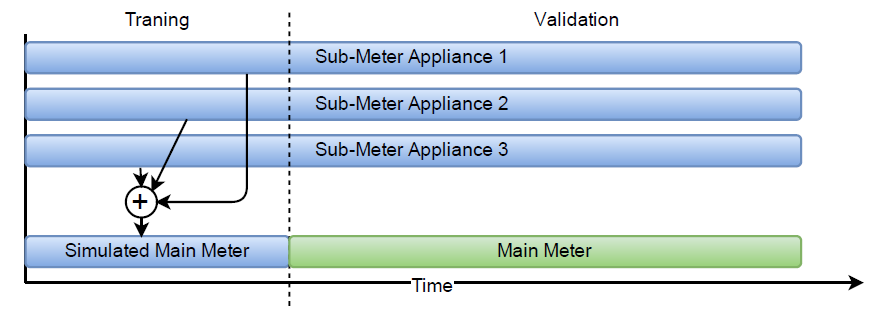
\includegraphics[width=0.9\textwidth]{billeder/SIMREAL.png}
\caption{Illustration of dataset creation by combining constructed and real data}
\label{fig:SHGSIMREAL}
\end{figure}

By training the model on the constructed data, is the true model for the appliances found. If the appliance noise in the real noisy environment is non-interfering can a performance like for the noise free environment described in section \ref{sec:NOISEFREE} be expected. 


\begin{table}[H]                             
\centering                                   
\begin{tabular}{lc|c|c|c|c|}
\cline{3-6}
                                                &        & \multicolumn{2}{c|}{FHMM} & \multicolumn{2}{c|}{Parson} \\ \cline{3-6} 
                                                &        & F1        & Accuracy      & F1         & Accuracy       \\ \hline
\multicolumn{1}{|l|}{\multirow{3}{*}{House 3}}  & TV 1   & 0.10      & 0.42          & 0.10       & 0.45           \\ \cline{2-6} 
\multicolumn{1}{|l|}{}                          & PC     & 0.13      & 0.39          & 0.12       & 0.44           \\ \cline{2-6} 
\multicolumn{1}{|l|}{}                          & TV 2   & 0.21      & 0.35          & 0.20       & 0.11           \\ \hline
\multicolumn{1}{|l|}{\multirow{4}{*}{House 10}} & TV 1   & 0.40      & 0.25          & 0.40       & 0.25           \\ \cline{2-6} 
\multicolumn{1}{|l|}{}                          & Stereo & -         & 1.00          & -          & 1.00           \\ \cline{2-6} 
\multicolumn{1}{|l|}{}                          & PC     & -         & 0.99          & -          & 0.99           \\ \cline{2-6} 
\multicolumn{1}{|l|}{}                          & TV 2   & -         & 0.99          & -          & 0.99           \\ \hline
\multicolumn{1}{|l|}{\multirow{3}{*}{House 18}} & TV 1   & 0.27      & 0.26          & 0.24       & 0.14           \\ \cline{2-6} 
\multicolumn{1}{|l|}{}                          & Lamp   & -         & 0.99          & -          & -              \\ \cline{2-6} 
\multicolumn{1}{|l|}{}                          & TV 2   & 0.73      & 0.58          & 0.73       & 0.58           \\ \hline
\end{tabular}                              
\caption{Disaggregation in constructed and real main meters combined}                     
\label{table:Tab:SHGSIMREAL}                 
\end{table}     

The results are shown in table \ref{table:Tab:SHGSIMREAL}. Here we see that the performance of this system is lower than the one from the noise free experiment. This lead to the conclusion that the noise is both affecting the models, and interfering in the validation process.  

The results from the disaggregation of the data in the real environment from section \ref{sec:NOISE} is compared with the results from the the experiments, where the models was extracted from constructed, data validated on the real data, is shown in table \ref{table:Tab:RealVsCon}. 

\begin{table}[H]                             
\centering                                   
\begin{tabular}{ccccccc}
\cline{3-4} \cline{6-7}
\multicolumn{1}{l}{}                            & \multicolumn{1}{c|}{}       & \multicolumn{2}{c|}{FHMM}                                 & \multicolumn{1}{c|}{} & \multicolumn{2}{c|}{FHMM}                                 \\
\multicolumn{1}{l}{}                            & \multicolumn{1}{c|}{}       & \multicolumn{2}{c|}{Real}                                 & \multicolumn{1}{c|}{} & \multicolumn{2}{c|}{Constructed}                          \\ \cline{3-4} \cline{6-7} 
\multicolumn{1}{l}{}                            & \multicolumn{1}{c|}{}       & \multicolumn{1}{c|}{F1}   & \multicolumn{1}{c|}{Accuracy} & \multicolumn{1}{c|}{} & \multicolumn{1}{c|}{F1}   & \multicolumn{1}{c|}{Accuracy} \\ \cline{1-4} \cline{6-7} 
\multicolumn{1}{|c|}{\multirow{3}{*}{House 3}}  & \multicolumn{1}{c|}{TV 1}   & \multicolumn{1}{c|}{0.19} & \multicolumn{1}{c|}{0.74}     & \multicolumn{1}{c|}{} & \multicolumn{1}{c|}{0.10} & \multicolumn{1}{c|}{0.42}     \\ \cline{2-4} \cline{6-7} 
\multicolumn{1}{|c|}{}                          & \multicolumn{1}{c|}{PC}     & \multicolumn{1}{c|}{0.19} & \multicolumn{1}{c|}{0.84}     & \multicolumn{1}{c|}{} & \multicolumn{1}{c|}{0.13} & \multicolumn{1}{c|}{0.39}     \\ \cline{2-4} \cline{6-7} 
\multicolumn{1}{|c|}{}                          & \multicolumn{1}{c|}{TV 2}   & \multicolumn{1}{c|}{0.03} & \multicolumn{1}{c|}{0.84}     & \multicolumn{1}{c|}{} & \multicolumn{1}{c|}{0.21} & \multicolumn{1}{c|}{0.35}     \\ \cline{1-4} \cline{6-7} 
\multicolumn{1}{l}{}                            &                             &                           &                               &                       &                           &                               \\ \cline{1-4} \cline{6-7} 
\multicolumn{1}{|c|}{\multirow{4}{*}{House 10}} & \multicolumn{1}{c|}{TV 1}   & \multicolumn{1}{c|}{0.60} & \multicolumn{1}{c|}{0.76}     & \multicolumn{1}{c|}{} & \multicolumn{1}{c|}{0.40} & \multicolumn{1}{c|}{0.25}     \\ \cline{2-4} \cline{6-7} 
\multicolumn{1}{|c|}{}                          & \multicolumn{1}{c|}{Stereo} & \multicolumn{1}{c|}{-}    & \multicolumn{1}{c|}{1.00}     & \multicolumn{1}{c|}{} & \multicolumn{1}{c|}{-}    & \multicolumn{1}{c|}{1.00}     \\ \cline{2-4} \cline{6-7} 
\multicolumn{1}{|c|}{}                          & \multicolumn{1}{c|}{PC}     & \multicolumn{1}{c|}{-}    & \multicolumn{1}{c|}{0.99}     & \multicolumn{1}{c|}{} & \multicolumn{1}{c|}{-}    & \multicolumn{1}{c|}{0.99}     \\ \cline{2-4} \cline{6-7} 
\multicolumn{1}{|c|}{}                          & \multicolumn{1}{c|}{TV 2}   & \multicolumn{1}{c|}{-}    & \multicolumn{1}{c|}{0.99}     & \multicolumn{1}{c|}{} & \multicolumn{1}{c|}{-}    & \multicolumn{1}{c|}{0.99}     \\ \cline{1-4} \cline{6-7} 
\multicolumn{1}{l}{}                            &                             &                           &                               &                       &                           &                               \\ \cline{1-4} \cline{6-7} 
\multicolumn{1}{|c|}{\multirow{3}{*}{House 18}} & \multicolumn{1}{c|}{TV 1}   & \multicolumn{1}{c|}{0.36} & \multicolumn{1}{c|}{0.65}     & \multicolumn{1}{c|}{} & \multicolumn{1}{c|}{0.27} & \multicolumn{1}{c|}{0.26}     \\ \cline{2-4} \cline{6-7} 
\multicolumn{1}{|c|}{}                          & \multicolumn{1}{c|}{Lamp}   & \multicolumn{1}{c|}{-}    & \multicolumn{1}{c|}{0.99}     & \multicolumn{1}{c|}{} & \multicolumn{1}{c|}{-}    & \multicolumn{1}{c|}{0.99}     \\ \cline{2-4} \cline{6-7} 
\multicolumn{1}{|c|}{}                          & \multicolumn{1}{c|}{TV 2}   & \multicolumn{1}{c|}{0.73} & \multicolumn{1}{c|}{0.58}     & \multicolumn{1}{c|}{} & \multicolumn{1}{c|}{0.73} & \multicolumn{1}{c|}{0.58}     \\ \cline{1-4} \cline{6-7} 
\end{tabular}                         
\caption{Trained in real vs. constructed data}                     
\label{table:Tab:RealVsCon}                    
\end{table}  

The tables shows that the performance of the system is better when trained in the real environment, as in relation to when the the system is trained in a noise free environment and than deployed in a noisy environment. This is in contrast to what one might think, since the noise free environment should have supplied more correct models. But when the appliance noise is removed from a house in the training process is a bias error introduced. 

Appliances such as refrigerators and freezers that are always on will create a local house bias. This will vary from house to house, and is depended on the types and number of appliances in the house. If only a small number of devices is modelled in each house, as the smartHG case, is the bias almost exclusivity a part of the appliance noise. When the models are fitted by training in the real data, is the bias learned into the model, and further improves the model. This is not the case when the model are trained in the constructed dataset. 

If not all appliances in a house is known, a better performance can therefore be obtained by training in the intended environment of deployment. 

Some algorithms are designed to not be affected by the house bias, and is therefore moved from different environments more easily. The Parson algorithm is designed with this in mind. The performance of the parson algorithm is therefore the same, or in some cases improved, when using models trained in constructed data. This advantage unfortunately comes with the problem of generalization, which lead to harder source separation, as discussed in section \ref{sec:NOISE}. 


\section{ Model Size And Completeness Influence }
Some of the parameters that often differ in the many different environments \ab{NILM} applications are deployed in, is the number of appliances in the environment, and the number of appliances that are known in the environment.  

The model size or complexity is a parameter that tells how many devices that are in a given environment. As the complexity in a \ab{NILM} application is increasing the detection rate is deceasing\citep{RefWorks:34}. This is one of the major problems and is why many researchers only focus on a small subset of appliances that have a fairly unique consumption signature. 

The model completeness is a metric describing how many appliances is known by the application in relation to the total amount of appliances. This can also be seen as the amount of appliance noise as discussed in section \ref{sec:AppNoise}.

\subsection{Test Set Creation}
\label{sec:datasetCreation}
In order to experiment with the completeness and complexity in the smartHG dataset, a more controllable series of datasets was artificially constructed from the smartHG dataset. 

First an artificial house was created called the "TV House" dataset. The TV house dataset is created by picking the relative dominant TV signals from the houses 5,10,11,13,18 and 23 in the smartHG dataset and combining them two one artificial house with 7 TV's. 

This dataset contains of dominant appliances, and there is no appliance noise from unknown devices. It is still worth noticing that all the 7 appliances is a Type-II appliances, and they are all TV's, which make there usage pattern some what similar. Since the Parson algorithm is greatly effected by this will the focus mainly be on the \ab{FHMM} algorithm. 

If the TV House dataset was seen as a set of sub-meters as mathematically shown in equation \ref{EQ:SUBMS}. 

\begin{equation}
	H_{full} = \{ TV_1, TV_2, ... , TV_7 \}
	\label{EQ:SUBMS}
\end{equation}

Since there is no appliance noise the main meter data can be found as the sum of sub-meters data as shown in equation \ref{EQ:SUMSUB}. 

\begin{equation}
	M_{main} = \sum_{X \in H_{full}}X
	\label{EQ:SUMSUB}
\end{equation}

Using this information it is possible to create a set with a specified complexity, by taking a subset of the $H_{full}$ set with the cardinality of the specified complexity. The main meter can now be found on this subset using the same principle as in equation \ref{EQ:SUMSUB}. Using the equation \ref{EQ:TVCARSET}, it is possible to find a set of all sets with a desired complexity $c$.

\begin{equation}
	\textbf{H}_c = \{ x | x \in \powerset{H_{full}}, \forall |x| = c   \}
	\label{EQ:TVCARSET}
\end{equation}

This can be graphically shown as in figure \ref{fig:PSILLU}. 

\begin{figure}[H]
\begin{picture}(0,200)
\put(0,0){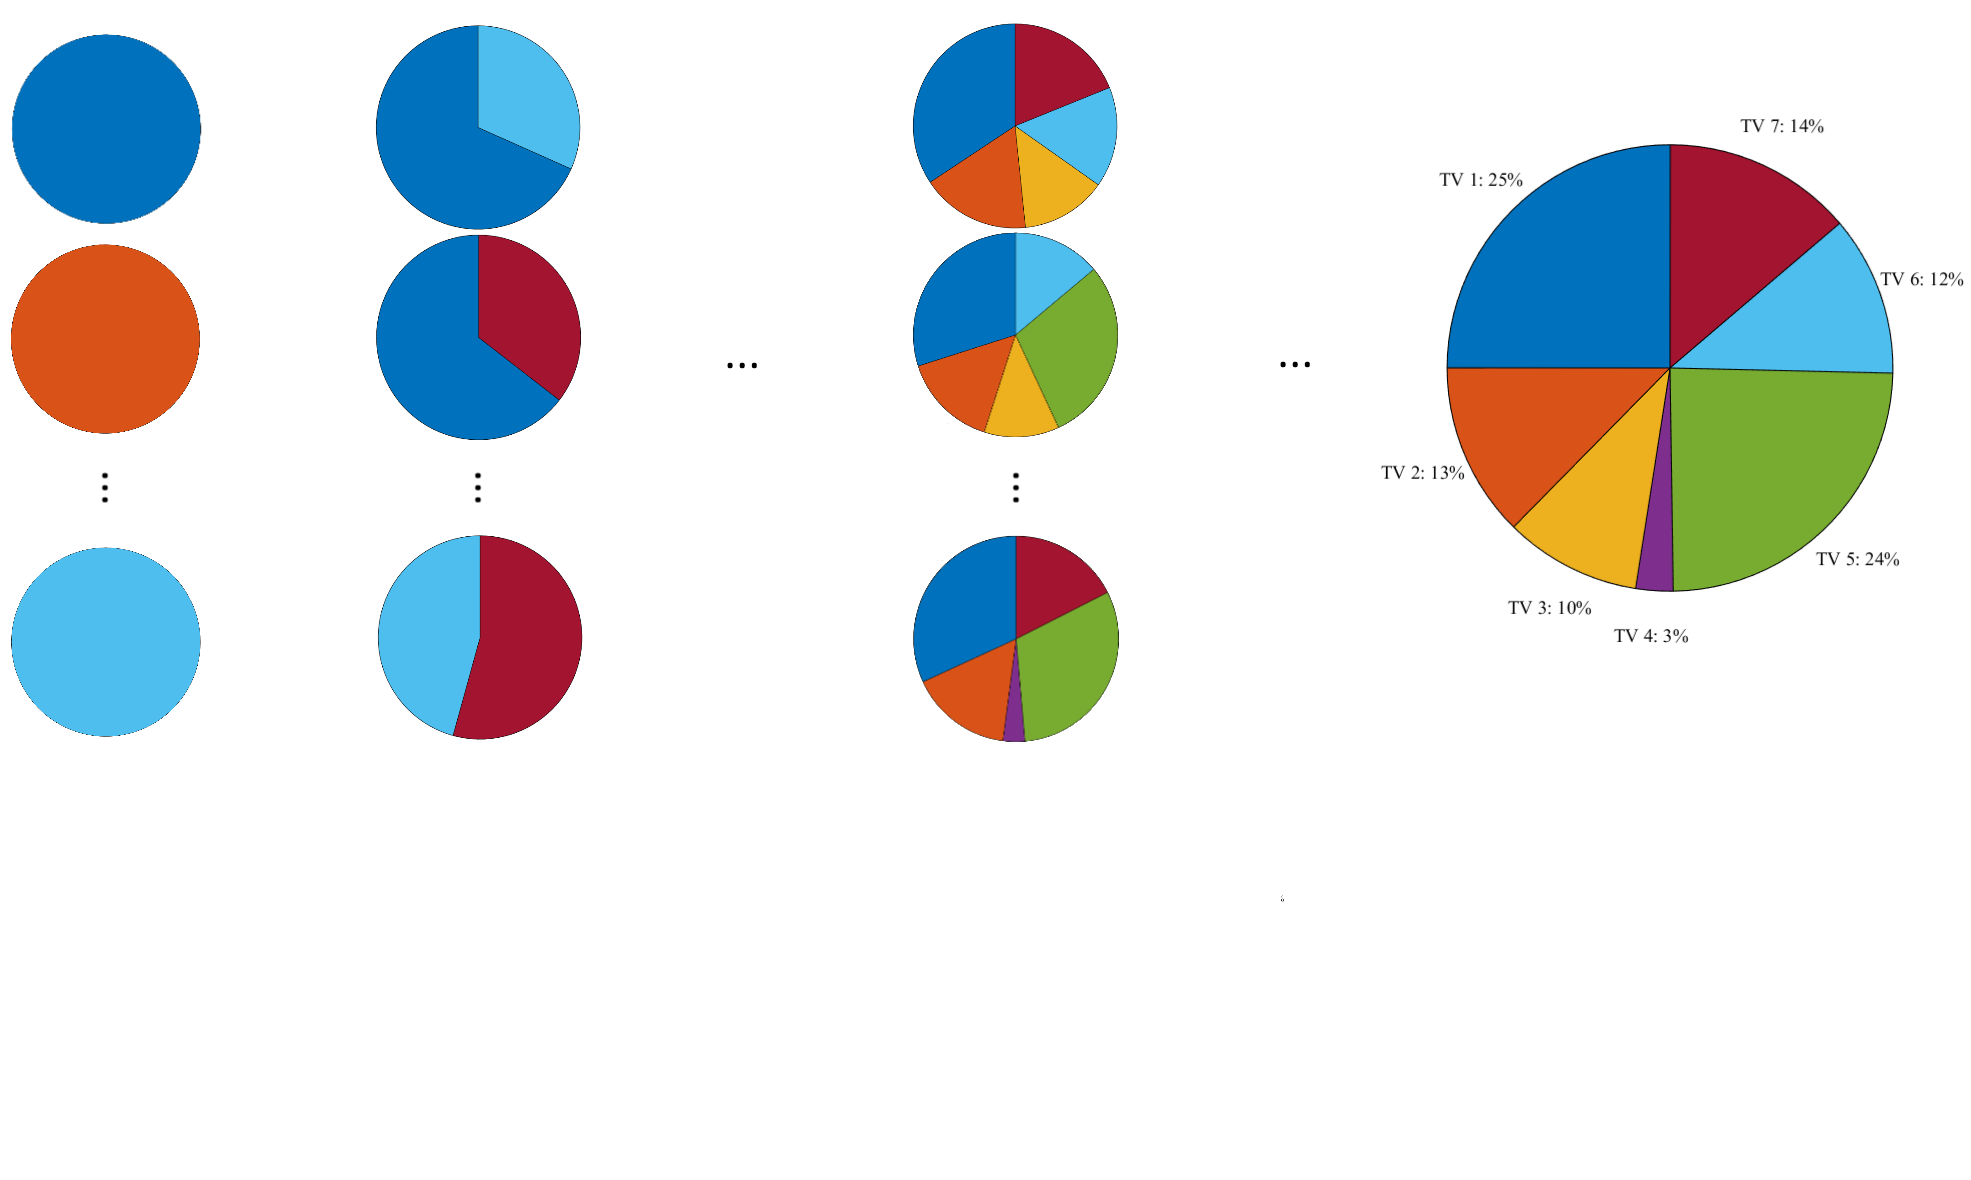
\includegraphics[width=1\textwidth]{billeder/CombiShow.png}}

\put(20,10){$\textbf{H}_1$}
\put(105,10){$\textbf{H}_2$}
\put(230,10){$\textbf{H}_5$}
\put(375,10){$\textbf{H}_7$}

\end{picture}
\caption{}
\label{fig:PSILLU}
\end{figure}

Where the $\textbf{H}_7$ only contains the $H_{full}$ set. In this manner it is possible to artificially create one or more datasets in a desired complexity equal to or less than the $H_{full}$ complexity. The amount of artificiality created houses for a given complexity can be found by using the simple combinatorial equation shown in equation \ref{EQ:nCr}.

\begin{gather}
		|\textbf{H}_c| = \frac{|H_{full}|!}{c! \times (|H_{full}| - c)!} \label{EQ:nCr} \\
		A_c = |\textbf{H}_c| \times \frac{c}{|H_{full}|} \label{EQ:ACr}
\end{gather}
% n! / ( r! (n - r)! )


As illustrated on figure \ref{fig:PSILLU} can an appliance appear in multiple sets in a given $\textbf{H}_c$ collection. The number of sets containing a specific appliance in a $\textbf{H}_c$ collection $A_c$ can be calculated as in equation \ref{EQ:ACr}. In order to ensure that the combination of appliances does not have a effect on the experiments, is the experiments conducted on all combinations in $\textbf{H}_c$. The results for each experiment is a average of the performance for the appliance in the experiment. 

\begin{table}[]
\centering
\begin{tabular}{c|c|c|c|c|c|c|c|}
\cline{2-8}
                       & $c = 1$ & $c = 2$ & $c = 3$ & $c = 4$ & $c = 5$ & $c = 6$ & $c = 7$ \\ \hline
\multicolumn{1}{|c|}{$|\textbf{H}_c|$} &    7   &    21   &    35   &    35   &   21    &   7    &    1  \\ \hline
\multicolumn{1}{|c|}{$A_c$} &    1   &     6  &     15  &     20  &    15   &    6   &    1   \\ \hline
\end{tabular}
\caption{TV House dataset complexity}
\label{Tab:TvHouse}
\end{table}

In the case of the TV house dataset can the $|\textbf{H}_c|$ and $A_c$ values for the different complexity be seen in table \ref{Tab:TvHouse}.


\subsection{Model Complexity Test}
To investigate the effect the number of appliances in a house, have on the performance of a \ab{NILM} system, is disaggregation done on every artificial house in $\textbf{H}$.

\begin{figure}[H]
\centering
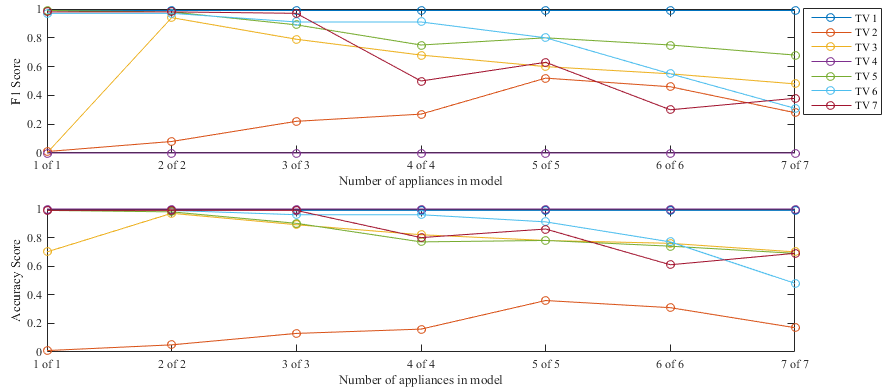
\includegraphics[width=1\textwidth]{billeder/ModelSize.png}
\caption{Average score at different complexity }
\label{fig:COMPT}
\end{figure}

The test is preformed on every combination, to ensure that there is not some combination that are more favourable than others. The results shown in figure \ref{fig:COMPT} is the average of the results from the many combinations as described in section \ref{sec:datasetCreation}. 

For the most part it is fairly easy to correctly classify the TV's when the complexity is only one. As a general trend does the F1 and accuracy score of the TV's decrees as the complexity of the house increase. This is due to the application spill over effect. The spill over effect is when there actually is an event, but the system classifies it to the wrong device.  An effect of this is most clearly seen on TV 2 signal. TV 2 is a very complex signal, and is therefore hard to track by the algorithm, as seen at the $\textbf{H}_1$ complexity that have a F1 score on almost zero. When the complexity is increased it looks like it is easier to detect the signal, and the F1 score is increasing. What is actually happening is the spill effect from the other TV's. Since all the appliances are TV's they have a lot of overlap in their usage, since a lot of people watches TV between 18-22. This makes the algorithm encounter signal's that are similar in structure for the different TV's, and it have a hard time deciding which appliance is responsible. Therefore can some of the events generated by the other TV's spill over in TV 2. If by chance TV 2 actually was on when the events from the other TV's was wrongfully assigned, the F1 and accuracy score of TV 2 would improve. 

For other appliances that are not as hard to classify as TV 2 will the spill over effect decrease the F1 and accuracy score as seen on the figure. 

\subsection{ Model Completeness Influence }



\begin{figure}[H]
\centering
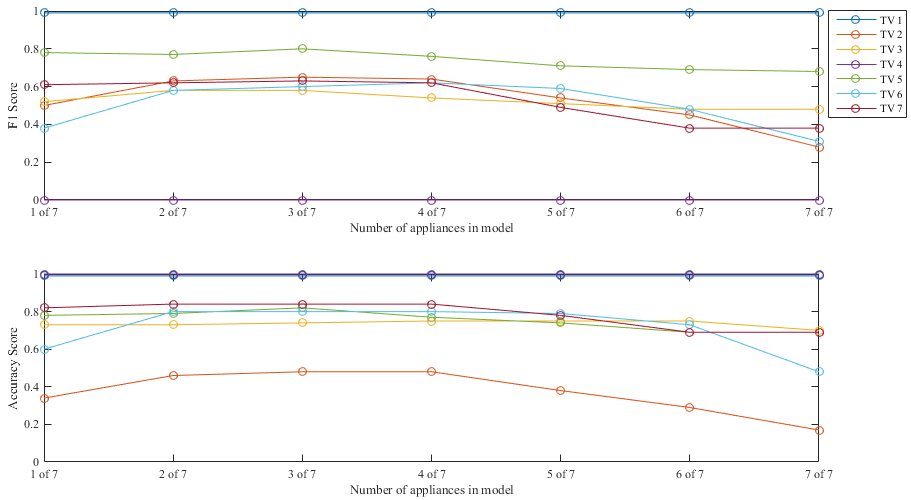
\includegraphics[width=1\textwidth]{billeder/ModelCompletness.png}
\caption{}
\end{figure}